% Cuerpo de la seccion "Aprender cuando dejar de copiar" (\input desde ASRN_Calvario_2026_es.tex).
% Fuentes: results/citas (CPU, la corrida principal), results/citas_a100 (su replicacion en la A100),
% docs/TECHNICAL_REPORT_es.md (seccion 7.2). Programa: benchmarks/experimento_citas.py.

Copia y MQAR no pueden poner a prueba los mecanismos de regulación: toda posición evaluada pide una copia, así que la
recuperación es todo lo que necesitan, y ahí la puerta, el reloj y las señales de Hawkes y de racha solo mostraron no
ser intrusivos (con ellos ASRN copia con 4$\times$ al 99.99\% y al 99.98\% en las 2 de 3 semillas que aprendieron y
llega a 99.75\% en MQAR con 4$\times$ los pares; sección~\ref{sec:ablation}). Su trabajo, decidir si copiar y cuándo
parar, importa al escribir libremente, así que su papel activo se prueba ahí, en un texto cuyas citas tienen un largo
acotado.

\paragraph{Montaje.} El texto son piezas al azar ($V=64$) en las que, con probabilidad 0.04 por posición, se cita un
trozo de las últimas 200 piezas de largo uniforme entre 6 y 12; en el texto real el 15.6\% de las piezas es
citado, y las rachas de grupos de 4 piezas ya vistos rara vez pasan de 9 piezas (lo hace el 0.9\%; la más larga es de
10). Se entrenan cinco modelos con la misma semilla, los mismos datos y la misma receta ($d=64$, dos bloques locales y
una capa ASRN, $L=256$, lote 16, tasa de aprendizaje $3\cdot10^{-3}$, 6{,}000 pasos con texto fresco): la capa completa
de 1.0; la capa sin las señales de Hawkes y de racha (congeladas en sus valores neutros); una puerta que solo ve el
estado oculto; sin puerta (fija en 1); y sin reloj ($\beta=\alpha=1$, $\gamma=0$). Cada uno escribe 128 piezas después
de inicios de 128 piezas de 64 textos de validación ($T=0.8$ con top-$k=40$ por omisión, y $T=1$; con y sin la memoria
de lo ajeno). Medimos la fracción de piezas escritas que cierran un grupo de 4 ya visto (\emph{citado}) y el largo de
las series seguidas de esas piezas (\emph{rachas}), juntando las semillas 0, 1 y 2. La corrida principal es en CPU
(\nolinkurl{results/citas/}); el banco de la A100 la repitió (\nolinkurl{results/citas_a100/}).

\begin{figure}[t]
\centering
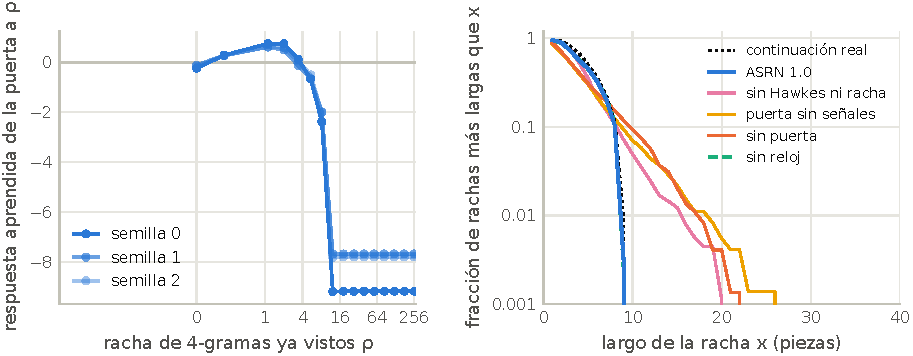
\includegraphics[width=0.94\linewidth]{citas.pdf}
\caption{Experimento de citas acotadas, corrida en CPU. Izquierda: la respuesta aprendida $f(\rho)$ de la puerta de la
capa completa a la racha de repetición $\rho$, tres semillas (eje logarítmico simétrico; nodos equiespaciados en
$\log(1+\rho)$ hasta 256). Derecha: fracción de las rachas escritas de más de $x$ piezas, juntando las tres semillas,
con el muestreo por omisión ($T=0.8$, top-$k=40$, memoria de lo ajeno activada); la curva sin el reloj casi coincide
con la de la capa completa.}
\label{fig:quote}
\end{figure}

\begin{table}[t]
\centering\small
\setlength{\tabcolsep}{3.3pt}
\begin{tabular}{lrrlrlrl}
\toprule
& \multicolumn{5}{c}{CPU (corrida principal)} & \multicolumn{2}{c}{replicación en la A100}\\
\cmidrule(lr){2-6}\cmidrule(lr){7-8}
& & & máx. & & & & máx.\\
Texto & citado & media & (por semilla) & $>9$ & pérdida val. & $>9$ & (por semilla)\\
\midrule
Continuación real & 15.6\% & 5.60 & 10 & 0.9\% & --- & 0.9\% & 10\\
\textbf{ASRN 1.0 (completa)} & \textbf{20.9\%} & \textbf{5.24} & \textbf{10} (9/10/10) & \textbf{0.3\%} &
3.7027--3.7056 & \textbf{0.3\%} & \textbf{10} (9/10/10)\\
sin Hawkes ni racha & 19.0\% & 5.22 & 21 (21/20/20) & 7.2\% & 3.7070--3.7079 & 7.9\% & 19 (17/15/19)\\
puerta sin señales & 13.9\% & 4.69 & 27 (17/23/27) & 9.3\% & 3.7290--3.7586 & 9.2\% & 39 (24/21/39)\\
sin puerta & 14.7\% & 4.91 & 23 (19/21/23) & 11.8\% & 3.7320--3.7396 & 12.0\% & 21 (21/20/20)\\
sin reloj & 20.2\% & 5.25 & 10 (10/10/9) & 0.2\% & 3.7042--3.7053 & 0.4\% & 10 (9/10/9)\\
\bottomrule
\end{tabular}
\caption{Escritura con el muestreo por omisión, semillas 0--2 juntas. \emph{Citado}: fracción de piezas escritas que
cierran un grupo de 4 ya visto; \emph{media}, \emph{máx.}: largo de las rachas; $>9$: porcentaje de rachas de más de 9
piezas; pérdida de validación: rango sobre las semillas.}
\label{tab:quote}
\end{table}

\paragraph{Qué aprende la puerta.} Solo con la pérdida de modelado de lenguaje, la puerta de la capa completa aprende
casi la misma respuesta en las tres semillas (figura~\ref{fig:quote}, izquierda): un empujón a copiar cuando empieza una
cita ($+0.62$ a $+0.76$ con $\rho\approx1$), negativo hacia $\rho\approx5$, y un freno fuerte desde $\rho\approx12$
($-7.7$ a $-9.2$), plano hasta $\rho=256$: un ``acantilado'' justo después de la racha más larga de los datos. La
respuesta sube y después baja, algo que una función monótona de la racha no puede expresar.

\paragraph{Efecto al escribir.} Con el muestreo por omisión, la capa completa escribe rachas como las del texto real
(tabla~\ref{tab:quote}, figura~\ref{fig:quote}, derecha): la más larga es de 10 y el 0.3\% pasa de 9 piezas. Sin las
señales de Hawkes y de racha, la racha más larga se duplica a 20--21 por semilla y el 7.2\% pasa de 9 piezas, aunque el
modelo cita casi lo mismo y su pérdida de validación es solo 0.002--0.005 más alta: el freno no se ve en la pérdida,
solo en lo que el modelo escribe. Con una puerta que no ve las señales, o sin puerta, el modelo cita menos, tampoco sabe
parar y su pérdida de validación empeora 0.03--0.05; sin el reloj escribe como la capa completa. El orden se mantiene
en todas las condiciones de muestreo (racha más larga por semilla de 9--10 para la capa completa, hasta 11 con la
temperatura que conserva la cita apagada, contra 15--36 de las tres variantes), y con $T=0.8$ apagar esa temperatura
sube la fracción citada de 20.9\% a 27.6\% y las rachas de más de 9 piezas de 0.3\% a 2.8\%.

\paragraph{Replicación en la A100.} Las mismas 5 variantes, 3 semillas y 6{,}000 pasos en la GPU reproducen el
resultado (tabla~\ref{tab:quote}, derecha): en todas las condiciones de muestreo, la racha más larga por semilla de la
capa completa es de 9--12 (12 solo con la memoria de lo ajeno desactivada y $T=0.8$) y sin el reloj de 9--10, contra
14--24 sin Hawkes ni racha, 15--39 con una puerta sin señales y 18--31 sin puerta. La pérdida de validación es
0.001--0.004 más alta sin Hawkes ni racha y 0.025--0.045 más alta con una puerta sin señales o sin puerta, y la
respuesta de la puerta tiene la misma forma ($+0.64$ a $+0.75$ con $\rho\approx1.1$, $-7.65$ a $-8.41$ desde
$\rho\approx12.3$).

\paragraph{Alcance.} Es una sola tarea sintética con tres semillas, $d=64$ y una capa ASRN. Quita juntas las señales de
Hawkes y de racha, y las entradas de la puerta en bloque, así que valida la puerta y sus señales de repetición, no cada
señal por separado. El reloj no tiene un efecto medible aquí, como se espera en una tarea sin cambios de tema. Cuán
seguido \emph{empieza} una cita no está calibrado (la temperatura que conserva la cita cubre solo su continuación): la
capa completa cita el 20.9--22.2\% de las piezas con $T=0.8$ y el 9.3--11.2\% con $T=1$ (21.8--24.2\% y 10.1--11.8\% en
la A100), contra 15.6\% en el texto real.
